% !TEX root = ../thesis-example.tex
%
%************************************************
% Evaluation
%************************************************
\chapter{Evaluation und Auswertung}
\label{sec:Evaluation}

\section{Einführung}
\label{sec:Evaluation:Einfuehrung}

In vorherigen Kapitel haben wir unseren Lösungsansatz in der Springermedizin-Suche implementiert. Wir wissen nun wie und warum wir den Reranking-Algorithmus umgesetzt haben. Was wir bisher nicht wissen ist, wie gut er funktioniert. Mithilfe einer Evaluation wollen wir darum nun messen, wie gut die Suchergebnis-Qualität der aktuellen Springermedizin-Suche im Vergleich zur im Zuge dieser Arbeit entwickelten Lösung mit dem Reranking-Algorithmus ist. 

\subsubsection{Ziel der Evaluation}
\label{sec:Evaluation:Einfuehrung:Ziel}

Die Evaluation soll Informationen darüber liefern, wie viel Verbesserung der neue Lösungsansatz bringt. Aus den Ergebnissen wollen wir erkennen, was an dem Lösungsansatz geändert werden muss, damit die Suche wirklich gute Ergebnisse aus Sicht der User liefert und unter welchen Voraussetzungen, sie im Springermedizin-Umfeld eingesetzt werden kann.

\subsubsection{Methodik}
\label{sec:Evaluation:Einfuehrung:Methodik}
Wir werden durch fachliche Experten (Redakteure von Springermedizin) die Suchergebnisse von oft gesuchten Suchanfragen bewerten lassen. Dazu werden wir eine Testumgebung mit einem Evaluations-System und den beiden oben angesprochenen Suchvarianten aufbauen. Die Redakteure sollen bei der Evaluation zu jeder Suchanfrage die ersten zehn Suchergebnisse analysieren und anhand der Suchsnippets die Relevanz bewerten. Diese Analyse sollen sie jeweils einmal auf der aktuellen Springermedizin-Suche und einmal auf der Springermedizin-Suche mit dem Reranking-Algorithmus durchführen. Am Ende werden wir die Ergebnisse auswerten und einen Vergleich der beiden Suchvarianten machen. 

\section{Aufbau der Analyse}
\label{sec:Evaluation:Aufbau}

Mithilfe der Relevanz-Bewertungen wollen wir das Qualitätsmaß der Suchvarianten bestimmen. Dazu müssen wir zuerst die \glqq zuverlässigen\grqq{} Bewertungen mittels \textit{Kappa-Koeffizienten} filtern und dann mithilfe der \textit{nDCG-Metrik} auswerten. Der Prozess dazu sieht wie folgt aus:

\begin{figure}[H]
\centering
\vspace{-.5em}
\caption[Prozess der Datenaufbereitung und Metrik der Auswertung]{Prozess der Datenaufbereitung und Metrik der Auswertung}
\vspace{.5em}
\label{fig:SucheSpringerNature}
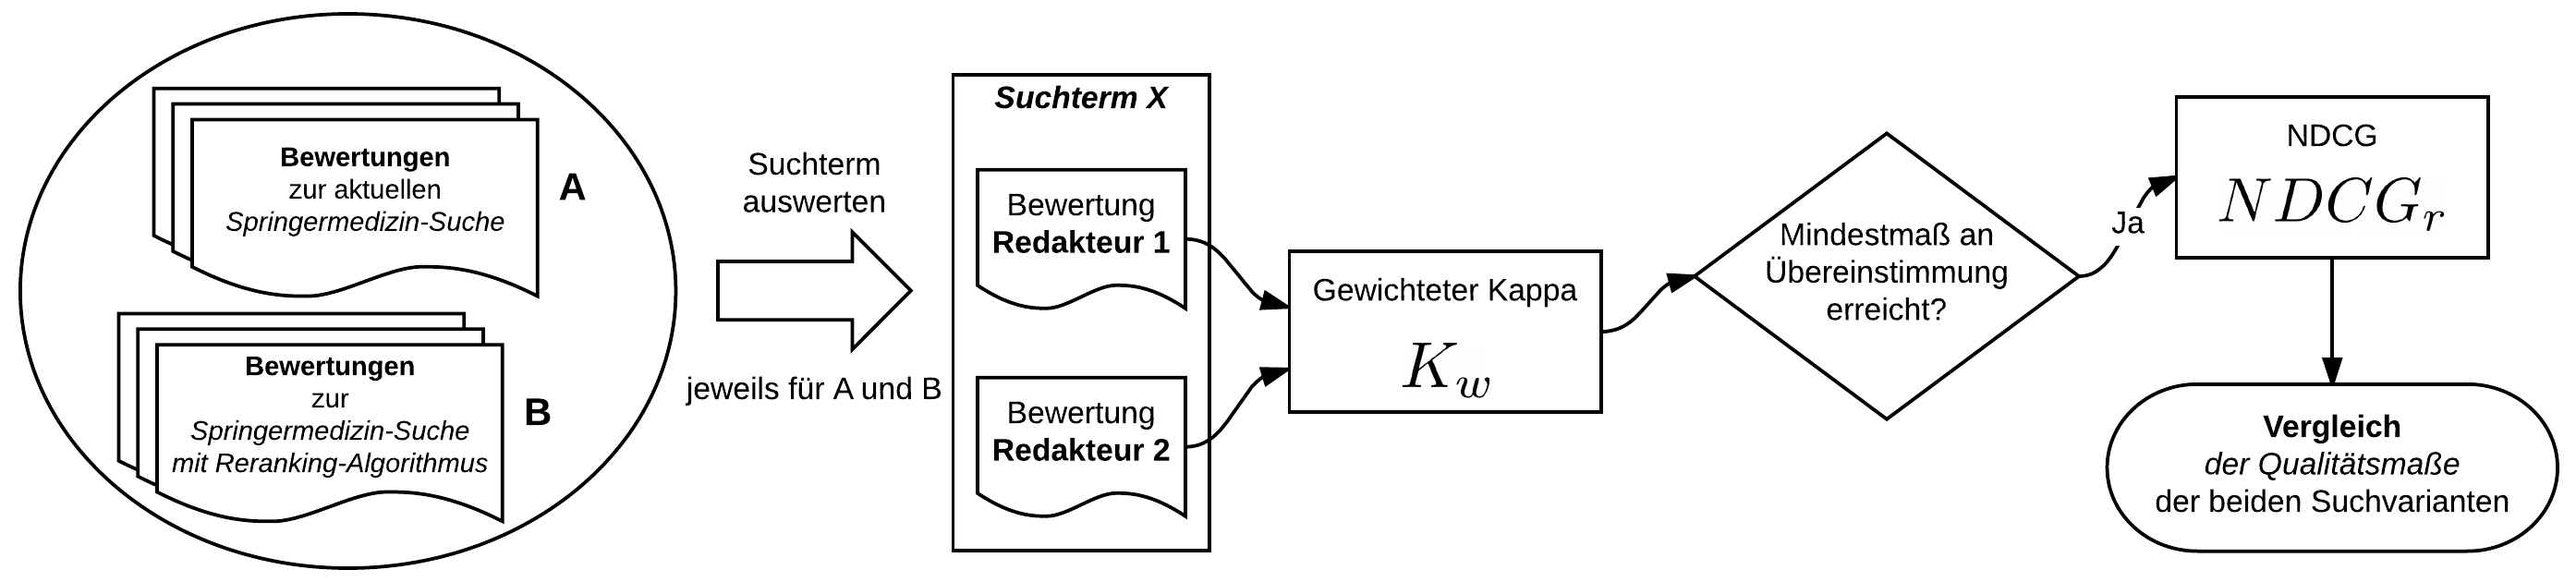
\includegraphics[width=\linewidth]{gfx/EvaluationDatenaufbereitung}
\vspace{-2em}
\end{figure}

\pagebreak

In diesem Kapitel werden Formeln eingeführt. Folgend eine Legende der wichtigsten Symbole:

\begin{table}[H]
\centering
\vspace{-.5em}
\caption[Legende der wichtigsten Formel-Symbolen für die Evaluation]{Legende der wichtigsten Formel-Symbolen für die Evaluation}
\label{tab:LegendeSymboleFormelnEvaluation}
\vspace{-.5em}
\footnotesize
\renewcommand*{\arraystretch}{1.2}
\resizebox{\textwidth}{!}{%
\begin{tabular}{llll}
\hline
\multicolumn{2}{l}{\textit{\textbf{Kappa}}}                            		& \multicolumn{2}{l}{\textit{\textbf{nDCG}}}                  \\ \hline
\textbf{Bedeutung} & \textbf{Symbol}                                   			& \textbf{Bedeutung} & \textbf{Symbol}                        \\ \hline
$K$				& Cohens-Kappa-Koeffizient                          				& $r$                	& die Anzahl der zu prüfenden Positionen \\
$p_0$			& Anteil tatsächlich beobachteter Übereinstimmungen 	& $i$                	& die zu prüfende Position               \\
$p_e$			& Anteil zufälliger Übereinstimmungen               			& $rel_i$				& Relevanz-Wert der Position $i$             \\
                   & 																						& $\vert REL \vert$				& die ideale Reihenfolge der Relevanz-Werte der Dokumente in $r$ \\
                   & 																						& $DCG_r$     		& Discounted Cumulative Gain             \\
                   &                                                   								& $IDCG_r$    		& Ideal Discounted Cumulative Gain       \\
                   &                                                   								& $nDCG_r$  		& Normalized Discounted Cumulative Gain  \\ \hline
\end{tabular}
}
\vspace{-2.5em}
\end{table}

\subsection{Datengrundlage}
\label{sec:Evaluation:Aufbau:Datengrundlage}

\subsubsection{Filterung der nutzbaren Daten mittels Cohens Kappa}
\label{sec:Evaluation:Aufbau:Datengrundlage:EvaluationsdatenFiltern}

Um die Zuverlässigkeit der Relevanz-Bewertungen zu messen, werden wir die gleichen Suchterme von jeweils zwei Redakteuren von Springermedizin bewerten lassen. Haben die Relevanz-Bewertungen ein zu geringes Maß an Übereinstimmung, sind sie für die anschliessenden Auswertungen zu wenig zuverlässig und werden darum in dieser nicht verwendet. Das meist verwendete Maß zur Bewertung der Übereinstimmungsgüte ist der \textit{Cohens-Kappa-Koeffizient} $K$~(siehe \cite{Kappa}). Dieser misst den Anteil \textit{übereinstimmender Bewertungen} $p_0$ und berechnet daraus die Zuverlässigkeit der Bewertung. Hierbei müssen wir berücksichtigen, dass die Beurteiler mit einer gewissen Wahrscheinlichkeit auch zufällig zur gleichen Einschätzung gelangen können. Der Cohens-Kappa-Koeffizient korrigiert das Maß an Übereinstimmung um diesen \textit{Zufallsfaktor} $p_e$. Die Berechnungsformel zur Bestimmung des Cohens-Kappa-Koeffizienten sieht wie folgt aus:

\vspace{-1.5em}
\begin{equation}	
	K = \frac{p_0 - p_e}{1 - p_e}
\end{equation}
\vspace{-1.5em}

\paragraph{Die Übereinstimmungen der beiden Redakteure aus einer Übereinstimmungsmatrix lesen}
Um die Stärke der Übereinstimmung der beiden Redakteuren bei der Relevanz-Bewertung eines Suchterms zu messen, erstellen wir zu jedem Suchterm eine Übereinstimmungsmatrix. Diese enthält die vier Relevanzstufen. Die Bewertungen der Suchergebnisse ordnen wir diesen vier Relevanzstufen zu:

\begin{table}[H]
\centering
\vspace{-.5em}
\caption[Übereinstimmungsmatrix von zwei Redakteuren bei der Klassifikation einer Suchanfrage]{Übereinstimmungsmatrix von zwei Redakteuren bei der Klassifikation einer Suchanfrage}
\label{tab:KreuztabelleKappaBerechnung}
\vspace{-.5em}
\resizebox{\textwidth}{!}{%
\setlength{\arrayrulewidth}{.5pt}
\renewcommand*{\arraystretch}{1.2}
\begin{tabular}{llcccccl}
\hhline{|*2{~}|*5{-}|}
                                                                                    & \multicolumn{1}{l|}{\textbf{}}                           & \multicolumn{4}{c|}{\cellcolor[HTML]{C0C0C0}\textbf{Redakteur 2}}                                                                                                                                                                      & \multicolumn{1}{c|}{\cellcolor[HTML]{C0C0C0}\textbf{Gesamt}}                                                                                  &                                 \\
                                                                                    & \multicolumn{1}{l|}{}                                    & \multicolumn{1}{c|}{\cellcolor[HTML]{C0C0C0}\textbf{-1}} & \multicolumn{1}{c|}{\cellcolor[HTML]{C0C0C0}\textbf{0}} & \multicolumn{1}{c|}{\cellcolor[HTML]{C0C0C0}\textbf{1}} & \multicolumn{1}{c|}{\cellcolor[HTML]{C0C0C0}\textbf{2}} & \multicolumn{1}{l|}{\cellcolor[HTML]{C0C0C0}}                                                                                                 &                                 \\ \hhline{|*7{>{\arrayrulecolor{black}}-}|~|}
\multicolumn{1}{|l}{\cellcolor[HTML]{C0C0C0}}                                       & \multicolumn{1}{l|}{\cellcolor[HTML]{C0C0C0}\textbf{-1}} & \multicolumn{1}{c|}{\cellcolor[HTML]{00D2CB}$a$}         & \multicolumn{1}{c|}{$b$}                                & \multicolumn{1}{c|}{$c$}                                & \multicolumn{1}{c|}{$d$}                                & \multicolumn{1}{c|}{$(a+b+c+d)/n$}                                                                                                            & \multicolumn{1}{c}{\textbf{$r_{-1}$}} \\ \hhline{|*1{>{\arrayrulecolor[HTML]{C0C0C0}}-}*6{>{\arrayrulecolor{black}}-}|}
\multicolumn{1}{|l}{\cellcolor[HTML]{C0C0C0}}                                       & \multicolumn{1}{l|}{\cellcolor[HTML]{C0C0C0}\textbf{0}}  & \multicolumn{1}{c|}{$e$}                                 & \multicolumn{1}{c|}{\cellcolor[HTML]{00D2CB}$f$}        & \multicolumn{1}{c|}{$g$}                                & \multicolumn{1}{c|}{$h$}                                & \multicolumn{1}{c|}{\cellcolor[HTML]{FFFFFF}$(e+f+g+h)/n$}                                                                                    & \multicolumn{1}{c}{\textbf{$r_0$}} \\ \hhline{|*1{>{\arrayrulecolor[HTML]{C0C0C0}}-}*6{>{\arrayrulecolor{black}}-}|}
\multicolumn{1}{|l}{\cellcolor[HTML]{C0C0C0}}                                       & \multicolumn{1}{l|}{\cellcolor[HTML]{C0C0C0}\textbf{1}}  & \multicolumn{1}{c|}{$i$}                                 & \multicolumn{1}{c|}{$j$}                                & \multicolumn{1}{c|}{\cellcolor[HTML]{00D2CB}$k$}        & \multicolumn{1}{c|}{$l$}                                & \multicolumn{1}{c|}{$(i+j+k+l)/n$}                                                                                                            & \multicolumn{1}{c}{\textbf{$r_1$}} \\ \hhline{|*1{>{\arrayrulecolor[HTML]{C0C0C0}}-}*6{>{\arrayrulecolor{black}}-}|}
\multicolumn{1}{|l}{\multirow{-4}{*}{\cellcolor[HTML]{C0C0C0}\textbf{Redakteur 1}}} & \multicolumn{1}{l|}{\cellcolor[HTML]{C0C0C0}\textbf{2}}  & \multicolumn{1}{c|}{$m$}                                 & \multicolumn{1}{c|}{$n$}                                & \multicolumn{1}{c|}{$o$}                                & \multicolumn{1}{c|}{\cellcolor[HTML]{00D2CB}$p$}        & \multicolumn{1}{c|}{$(m+n+o+p)/n$}                                                                                                            & \multicolumn{1}{c}{\textbf{$r_2$}} \\ \hhline{|*7{-}|}
\multicolumn{2}{|l|}{\cellcolor[HTML]{C0C0C0}\textbf{Gesamt}}                                                                                  & \multicolumn{1}{c|}{$(a+e+i+m)/n$}                       & \multicolumn{1}{c|}{$(b+f+j+n)/n$}                      & \multicolumn{1}{c|}{$(c+g+k+o)/n$}                      & \multicolumn{1}{c|}{$(d+h+l+p)/n$}                      & \multicolumn{1}{c|}{\cellcolor[HTML]{FFCB2F}\begin{tabular}[c]{@{}c@{}}$\textbf{n} = \sum \text{ aller Matrixelemente} \left( a,b...o,p \right)$ \end{tabular}} &                                 \\ \hhline{|*7{-}|}
                                                                                    &                                                          & \textbf{$c_{-1}$}                                              & \textbf{$c_0$}                                             & \textbf{$c_1$}                                             & \textbf{$c_2$}                                             & \multicolumn{1}{l}{}                                                                                                                          &                                
\end{tabular}%
}
\vspace{-2em}
\end{table}

Den Anteil tatsächlich beobachteter Übereinstimmungen $p_0$ können wir direkt aus den Werten der \textit{Hauptdiagonalen} der Matrix berechnen. Die Berechnungsformel dazu sieht wie folgt aus: 

\vspace{-1.5em}
\begin{equation}	
	p_0 = \frac{ \sum \text{ der Übereinstimmungen} \left( a + f + k + p \right)}{ \sum \text{ aller Übereinstimmungen} \left( n \right) }
\end{equation}
\vspace{-1em}

Der daraus resultierende Wert müssen wir um den Anteil zufälliger Übereinstimmungen $pe$ korrigieren. Der Wert von $pe$ wird mithilfe der Randsummen der Matrix (Spalten- bzw. Zeilensummen) berechnet. Dazu muss jede Randsumme zuerst durch $n$ dividiert werden. Danach wird zu jeder Kategorie das Produkt der Spalten und Zeilensumme gebildet, mit welchem anschließend die Summe der Kategorien berechnet wird. Die komplette Berechnungsformel von $pe$ sieht wie folgt aus:

\vspace{-1.5em}
\begin{equation}	
	p_e = \left(  \left(\frac{  r_{-1} }{ n } \cdot \frac{ c_{-1} }{ n } \right) +   \left(\frac{  r_0 }{ n } \cdot \frac{ c_0  }{ n } \right) +   \left(\frac{  r_1 }{ n } \cdot \frac{ c_1 }{ n } \right)  +  \left(\frac{ r_2 }{ n } \cdot \frac{   c_2 }{ n }\right) \right)
\end{equation}
\vspace{-2em}

\paragraph{Kappa-Koeffizienten gewichten um Abweichungen der Bewertungen in Relation zu derer Relevanzdifferenz zu stellen}
Relevanz-Bewertungen werden meist sehr subjektiv gefällt. Wir müssen darum davon ausgehen, dass die Redakteure häufig kleinere Abweichungen in den Bewertungen haben werden. Weichen sie mehrere Kategorien voneinander ab, sollten wir diese Abweichung schwerer wiegen als die, bei benachbarten Kategorien. Unsere bisherige Formel stuft alle Abweichungen gleich ein. Mithilfe der Erweiterung des Kappa-Koeffizienten um eine Gewichtung der Abweichungsstärke zwischen 0 und 1, können wir unsere Formel in das gewichtete Kappa $K_w$~(siehe \cite{KappaWerte}) transformieren. Dazu müssen wir bei der Berechnung der Spalten- und Zeilensummen \textit{die Anzahl der Kategorien}, die das Matrixelement zur Hauptdiagonalen abweicht, berücksichtigen und diese Abweichung gewichten. Für unsere Berechnung definieren wir die Gewichte wie folgt:

\begin{table}[H]
\centering
\vspace{-.5em}
\caption[Gewichtung der Abweichungsstärke einer Kategorie zur Hauptdiagonalen]{Gewichtung der Abweichungsstärke einer Kategorie zur Hauptdiagonalen}
\label{tab:GewichtungAbweichungenKappaBerechnung}
\vspace{-.5em}
\footnotesize
\renewcommand*{\arraystretch}{1.2}
\begin{tabular}{cl}
\hline
\multicolumn{1}{l}{\textbf{Gewichtung}} & \textbf{Anzahl Kategorien Abweichung} \\ \hline
\textit{0.25}                                     & 0 \textit{(auf Hauptdiagonal)}                 \\ 
\textit{0.5}                                      & 1 \textit{(benachbarte Kategorie)}             \\ 
\textit{0.75}                                     & 2                                     \\ 
\textit{1}                                        & 3                                     \\ \hline
\end{tabular}
\vspace{-1.5em}
\end{table}

\paragraph{Kappa interpretieren}

Wie in \cite{KappaWerte} beschrieben, müssen die Kappa-Werte individuell interpretiert werden. Es gibt jedoch Richtlinien. In \cite{Kappa} wird bei einem Kappa-Wert ab 0.60 von einer guten Übereinstimmung ausgegangen. Da wir bei unserer Evaluation nur mit einer begrenzten Anzahl von Bewertungen arbeiten können, müssen wir das Mindestmaß der Übereinstimmungsgüte anhand der Kappa-Koeffizienten der Bewertungen definieren. Wir werden es so definieren, dass wir mindestens 80 Prozent der Bewertungen auswerten können. Die unter dem Mindestmaß liegenden Bewertung werden wir in der Auswertung ignorieren. 

\subsection{Metrik}
\label{sec:Evaluation:Aufbau:Metrik}

\subsubsection{Qualitätsmaß einer Suchvariante bestimmen}
\label{sec:Evaluation:Aufbau:Metrik:QualitaetMessen}

In der Evaluation werden zu jedem Suchterm zwei Bewertungen für die aktuelle Springermedizin-Suche und zwei Bewertungen für die Springermedizin-Suche mit dem Reranking-Algorithmus abgegeben. Um das Qualitätsmaß einer Suche zu bestimmen, werden wir den \textit{Normalized Discounted Cumulative Gain} (nDCG, siehe \cite{nDCG}) verwenden. Der nDCG misst die Qualität des Rankings der Suche und wird in der Information Retrieval\footnote{Mit Information Retrieval werden Methoden und Verfahren, die der Aufbereitung und Speicherung von Wissen und der Gewinnung von Informationen dienen bezeichnet} oft eingesetzt um die Effektivität eines Such-Algorithmus zu messen.  Um das Qualitätsmaß der beiden in der Evaluation verwendeten Suchvarianten zum Suchterm zu bestimmen, berechnen wir zu jeder Suchvariante den nDCG der beiden Bewertungen des Suchterms. Nehmen wir den Mittelwert der beiden resultierenden nDCG-Werte, erhalten wir den effektiven nDCG-Wert. Die nDCG-Werte der beiden Suchvarianten können wir dann miteinander vergleichen.

\subsubsection{Evaluationsdaten mittels nDCG auswerten}
\label{sec:Evaluation:Aufbau:Metrik:EvaluationsdatennDCG}

Der nDCG verfolgt die Grundidee, Suchergebnislisten dahingehend zu untersuchen, ob Dokumente mit hoher Relevanz zum Suchterm vor denen mit weniger Relevanz stehen. Der nDCG vergleicht dazu die Relevanz der Dokumente mit ihrer Reihenfolge im Suchresultat. Diese Metrik macht für unseren Reranking-Algorithmus insofern Sinn, dass sie nicht von bestimmten Relevanz-Werten für die Suchresultate ausgeht, sondern wie unser Algorithmus sich nur auf die Reihenfolge der Relevanz-Werte konzentriert. 

\subsubsection{Berechnung des Qualitätsmaß einer Suchvariante mittels nDCG}
\label{sec:Evaluation:Aufbau:Metrik:BerechnungnDCG}

\paragraph{Der nDCG baut auf dem DCG auf} Um den nDCG-Wert zu bestimmen, müssen wir zuerst den \textit{Discount Cumulative Gain} (DCG) jeder Position des untersuchten Suchresultats berechnen. Der DCG zielt darauf ab, das Qualitätsmaß einer Suchergebnisliste herunterzustufen, wenn relevante Dokumente schlechter als weniger relevante positioniert sind. Die Formel des DCG wird wie folgt definiert:

\vspace{-1.5em}
\begin{equation}	
DCG_{r} = \sum\limits_{i=1}^r \frac{2^{rel_{i}} - 1}{\log_2(i+1)}
\end{equation}
\vspace{-1em}

Wie wir erkennen können, werden Dokumente umso geringer bewertet, je weiter hinten sie im Suchresultat erscheinen. Dafür sorgt $\log_2(i+1)$ als Divisor in der Summenfunktion, dessen Wert mit steigenden Dokumentposition größer wird.

\paragraph{Der DCG muss normalisiert werden, um das Qualitätsmaß einer Suche über unterschiedliche Anfragen zu bewerten}
Der DCG ist auf den Vergleich von Suchanfragen mit gleicher Resultatslänge ausgelegt. Haben die zu untersuchenden Suchanfragen eine unterschiedliche Anzahl der zu untersuchenden Positionen, variiert die maximal erreichbare Punktzahl. Der nDCG normalisiert diese Punktewerte, indem er die Reihenfolge der Relevanz-Werte des Suchergebnisses mit der \textit{idealen Reihenfolge} derselben Relevanz-Werte vergleicht. Die Formel des nDCG wird wie folgt definiert:

\vspace{-.25em}
\begin{spacing}{.25}
\begin{align}
  &&	nDCG_{r} &= \frac{DCG_r}{IDCG_r} &\\
  \intertext{wobei:}
  &&	IDCG_{r} 	&= \sum\limits_{i=1}^{\vert REL \vert} \frac{2^{rel_{i}} - 1}{\log_2(i+1)}
\end{align}
\end{spacing}
\vspace{.25em}

Der resultierende Ergebnis-Wert des $nDCG_r$ bewegt sich zwischen 0 und 1. Entspricht die Reihenfolge der Suchergebnisse, der Relevanz der Suchergebnisse, so gilt $DCG_r = IDCG_r$. Dies entspricht dem Idealfall, die Suche besitzt in diesem Fall den $nDCG_r$-Wert 1 und somit das maximal mögliche Qualitätsmaß für den getesteten Suchterm.

\subsection{Vorgehen}
\label{sec:Evaluation:Aufbau:Vorgehen}

\subsubsection{Testumgebung aufbauen}
\label{sec:Evaluation:Aufbau:Vorgehen:Aufbau}

Um eine Evaluation durchführen zu können, müssen wir eine passende Testumgebung aufbauen. Diese besteht aus einem Evaluations-System, einer Instanz der aktuellen Springermedizin-Applikation und einer Instanz des neu implementierten Lösungsansatzes. Auf dem Evaluations-System sollen fachliche Experten (Redakteure von Springermedizin) die Relevanz der Suchergebnisse der beiden Suchmaschinen vergleichen. Dazu sollen die jeweils ersten zehn Suchergebnisse nach Relevanz zum Suchterm bewertet werden. Der Ergebnisse werden in einer Datenbank gespeichert, um sie später auszuwerten. 

\paragraph{Aufbau des Evaluations-Systems}
Für die Analysen der Beurteiler implementieren wir selber ein kleines Evaluations-System als Web-Applikation. Das hat den Vorteil, dass wir selber definieren können, wie der Analyse-Prozess und wie die Datenstruktur der Analyse-Ergebnisse aussehen sollen. Das System umfasst eine Administrationsoberfläche zur Verwaltung der Analysedaten und eine Anwenderoberfläche, zur Analyse der zugeteilten Suchterme. Der Beurteiler soll nur seine, ihm zugeteilten Suchterm-Analysen sehen. Um Analysen durchführen zu können, muss sich der Beurteiler darum an der Applikation anmelden. So können wir jedem Beurteiler ein eigenes Profil anlegen und ihm seine zu analysierenden Suchterme zuweisen. 

\paragraph{Analyse eines Suchterms}
Wir wollen zu jedem Suchterm eine Bewertung der aktuellen Springermedizin-Suche und eine der Suche mit dem implementierten Reranking-Algorithmus. Wir bauen die Analysen darum so, dass der Benutzer beide Bewertungen nacheinander in derselben Analyse ausführt. Zur Bewertung implementieren wir ein Maske, bestehend aus der zu beurteilende Suchvariante und einem Formular zur Bewertung der ersten zehn Suchresultate des Suchergebnisses. Die Bewertung besteht aus einer Skala von vier Relevanz-Werten:

\begin{table}[H]
\centering
\vspace{-.5em}
\caption[Relevanz-Werte für Bewertung der Suchresultate]{Relevanz-Werte für Bewertung der Suchresultate}
\label{tab:RelevanzWerteBewertungEvaluation}
\vspace{-.5em}
\footnotesize
\renewcommand*{\arraystretch}{1.2}
\begin{tabular}{llc}
\hline
\textbf{Relevanz}            & \textbf{Beschreibung}           & \textbf{Relevanz-Wert} \\ \hline
\textit{not relevant}        & Ergebnis hat \textbf{\textit{gar keine}} Relevanz & -1 \\
\textit{moderately relevant} & Ergebnis ist \textbf{\textit{eher irrelevant}}    & 0 \\
\textit{relevant}            & Ergebnis ist \textbf{\textit{eher relevant}}      & 1 \\
\textit{highly relevant}     & Ergebnis ist \textbf{\textit{sehr relevant}}      & 2 \\ \hline
\end{tabular}
\vspace{-2em}
\end{table}

Ist eine Bewertung gespeichert, wird die zweite Variante der Suche geladen. Eine Analyse ist dann abgeschlossen, wenn beide Suchvarianten bewertet sind. Der gesamte Prozessablauf einer Analyse sieht wie folgt aus:

\begin{figure}[H]
\centering
\vspace{-.5em}
\caption[Analyseprozess für Bewertung einer Suchvariante]{Analyseprozess für Bewertung einer Suchvariante}
\vspace{.5em}
\label{fig:AnalysemaskeEvaluation}
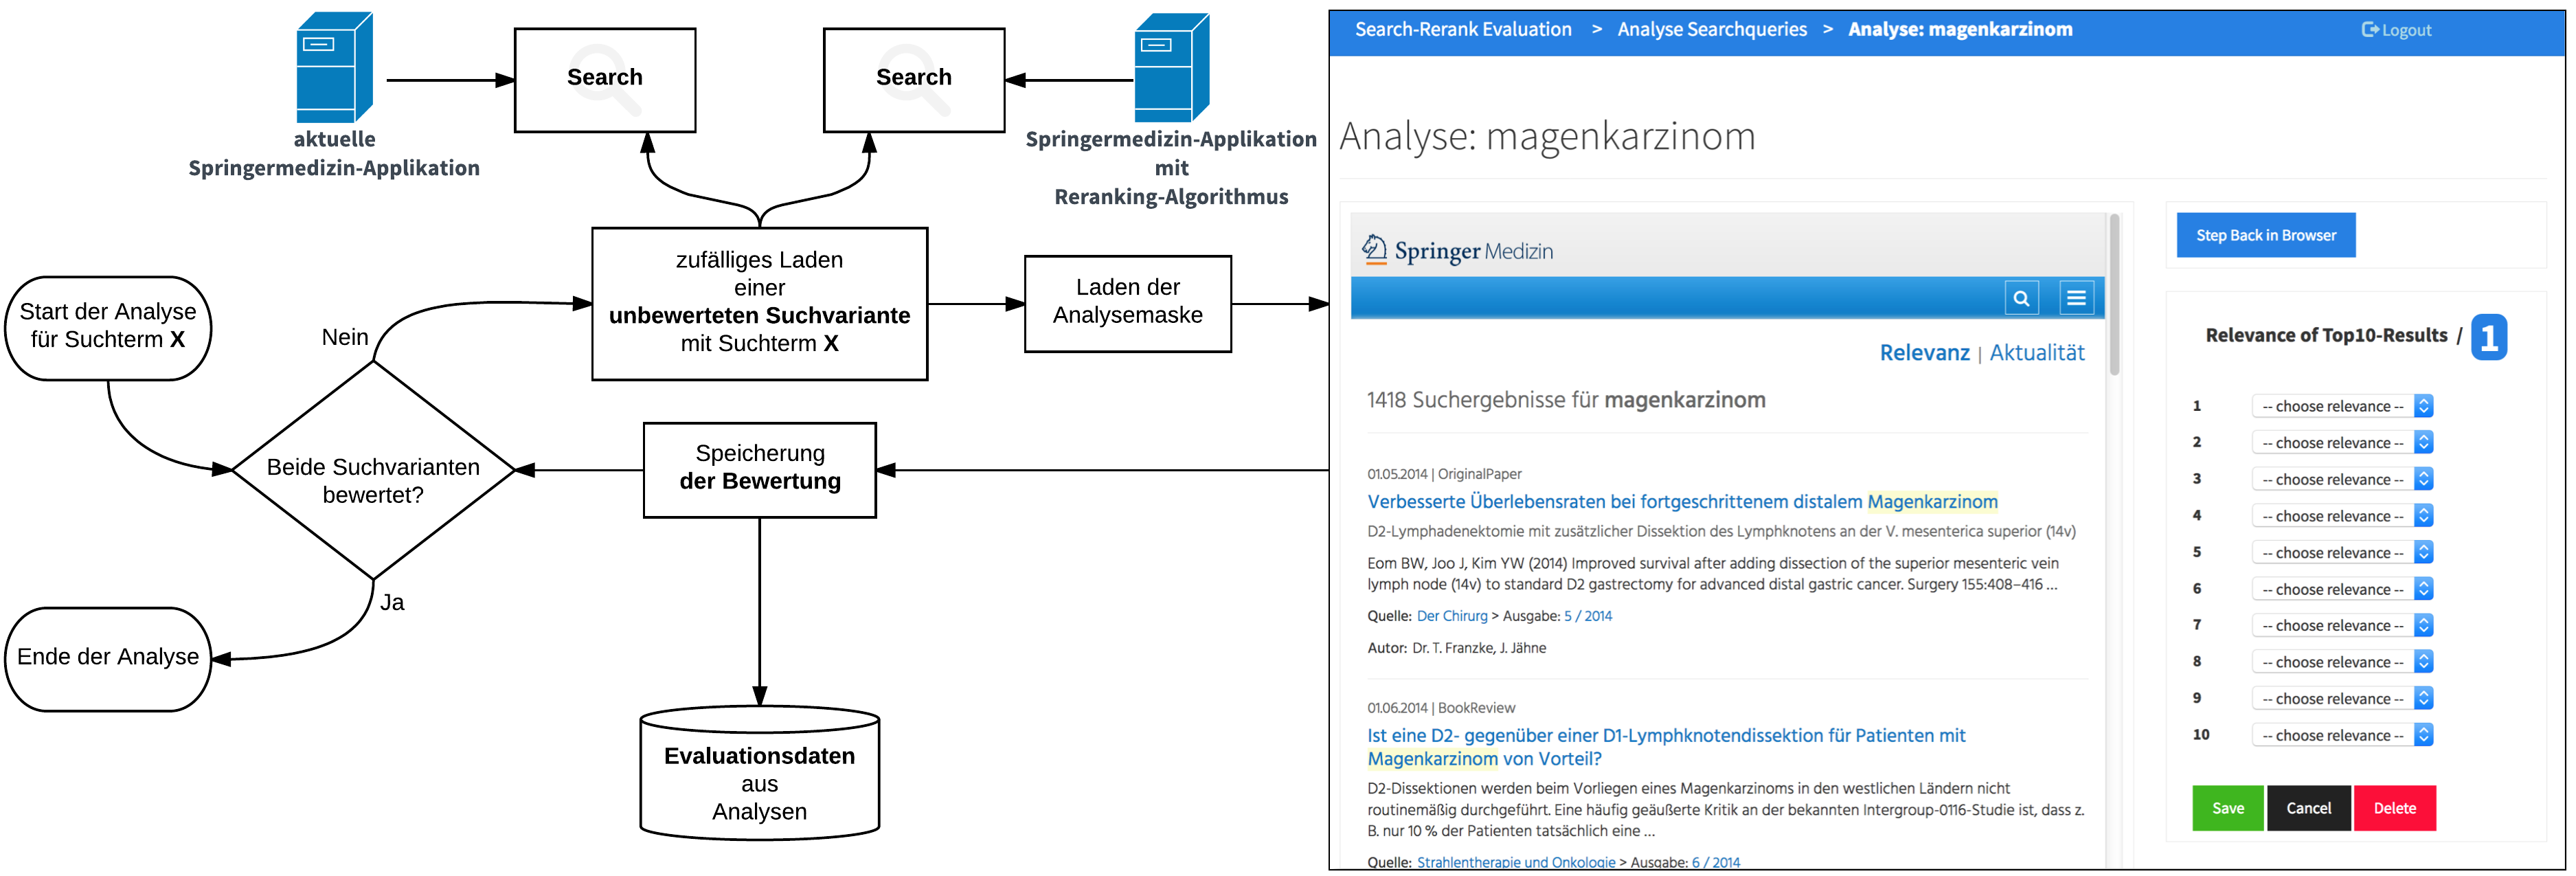
\includegraphics[width=\linewidth]{gfx/AnalysemaskeEvaluation}
\vspace{-1em}
\end{figure}

\subsubsection{Evaluations-Daten speichern}
\label{sec:Evaluation:Aufbau:Vorgehen:Speichern}

Zu jeder Analyse werden wir neben den Relevanz-Bewertungen und den Suchterm-Informationen auch wichtige Informationen zu den Click-Through-Daten und den Suchergebnissen speichern. Folgende Informationen liegen uns am Ende einer Analyse vor:

\begin{table}[H]
\centering
\vspace{-.5em}
\caption[Gespeicherte Evaluations-Daten zur Suchterm-Analyse]{Gespeicherte Evaluations-Daten zur Suchterm-Analyse}
\label{tab:EvaluationsDatenSpeicherung}
\vspace{-.5em}
\footnotesize
\renewcommand*{\arraystretch}{1.2}
\resizebox{\textwidth}{!}{%
\begin{tabular}{llll}
\hline
\textbf{Objekt}                                        & \textbf{Beide Suchvarianten}             & \textbf{Suche mit Reranking-Algorithmus} & \textbf{Beschreibung}                              \\ \hline
\multirow{4}{*}{\textit{\textbf{Analyse}}}             & \textit{Suchterm}                        & \textit{}                                & Analysierter Suchterm                              \\
                                                       & \textit{Beurteiler}                      & \textit{}                                & User-Informationen des Beurteilers                 \\
                                                       & \textit{Suchvariante}                    & \textit{}                                & Suche mit / ohne Reranking-Algorithmus             \\
                                                       & \textit{}                                & \textit{Wert des Zufallsfaktors}         & Einfluss-Wert Zufallsfaktor                        \\ \hline
\textit{\textbf{Bewertungen}}                          & \textit{Relevanz-Werte der Positionen}   & \textit{}                                & Relevanz-Bewertungen der ersten zehn Suchresultate \\ \hline
\multirow{2}{*}{\textit{\textbf{Click-Through-Daten}}} & \textit{}                                & \textit{User-Filter}                     & Alle Benutzer / eingeloggte Benutzer der Suche     \\
                                                       & \textit{}                                & \textit{Anzahl Klicks Gesamt}            & Anzahl gelesener Klicks aus Click-Through-Daten    \\ \hline
\textit{\textbf{Suchergebnis}}                         & \textit{Dokument-ID's der Suchresultate} & \textit{}                                & Dokument-ID's der ersten zehn Suchergebnisse       \\ \hline
\end{tabular}
}
\vspace{-2em}
\end{table}

\subsubsection{Evaluations-System auswerten}
\label{sec:Evaluation:Aufbau:Vorgehen:Auswerten}

Nach Abschluss der Evaluationsphase werden wir die Evaluations-Daten auswerten. Die Auswertung der Daten findet direkt im Evaluations-System statt. Dazu werden wir die Relevanz-Bewertungen aus der Datenbank lesen und wie oben beschrieben mit dem Cohens-Kappa-Koeffizienten und der nCDG-Metrik auswerten. Mithilfe der Evaluations-Daten können wir dann auch weitere Auswertungen zu den Click-Through-Daten und den Suchergebnissen der Suchterme machen.

\subsection{Durchführung}
\label{sec:Evaluation:Aufbau:Durchfuehrung}

\subsubsection{Zu analysierende Suchterme}
\label{sec:Evaluation:Aufbau:Durchfuehrung:Aufgabenstellung}

Um die Evaluation praxisrelevant und mit genügend Click-Through-Daten ausführen zu können, wurden die Suchanfragen der letzten zwei Monate auf der Springermedizin-Suche analysiert und 80 oft gesuchte Suchterme ausgewählt. Springermedizin hat ein breites Spektrum an medizinischen Fachgebieten. Um fachlich gute Bewertungen zu kriegen, haben wir die Suchterme nach Fachrichtung unterteilt und jeweils zwei Beurteilern zugeteilt, die aus der Fachrichtung kommen:

\begin{table}[H]
\centering
\vspace{-.5em}
\caption[Fachrichtungen der Suchterme der Evaluation]{Fachrichtungen der Suchterme der Evaluation}
\label{tab:FachrichtungenSuchtermeEvaluation}
\vspace{-.5em}
\footnotesize
\renewcommand*{\arraystretch}{1.2}
\resizebox{\textwidth}{!}{%
\begin{tabular}{llc}
\hline
\textbf{Fachrichtung}            		& \textbf{Medizinisches Gebiet / Medizinischer Zweig}                  	& \multicolumn{1}{l}{\textbf{Anzahl zugeteilte Suchterme}} \\ \hline
\textit{Onkologie}               		& Tumorerkrankungen                                                    					& 10                                                       \\ \hline
\textit{Zahnmedizin}             		& Fachgebiet der Zahn-, Mund- und Kieferheilkunde                      		& 20                                                       \\ \hline
\textit{Gynäkologie}             		& Spezifischen Erkrankungen des weiblichen Körpers                    		& 10                                                       \\ \hline
\textit{AINS}                    			& Anästhesiologie, Intensivmedizin, Notfallmedizin und Schmerztherapie & 10                                                       \\ \hline
\textit{Neurologie, Psychiatrie} 	& Erkrankungen des Nervensystems und der Psyche                        	& 10                                                       \\ \hline
\textit{Innere Medizin}          		& Erkrankungen der inneren Organe                                      			& 10                                                        \\ \hline
\textit{Orthopädie}              		& Aufbau der Knochen und Muskeln des Menschen                          	& \multirow{3}{*}{10}                                      \\
\textit{Urologie}               			& Erkrankungen der Niere, Harnblase, Harnleiter und Harnröhre         	&                                                          \\
\textit{HNO}               				& Hals-Nasen-Ohren-Heilkunde                                           				&                                                          \\ \hline
\textbf{Gesamt:}                 		& \textbf{}                                                            							& \textbf{80}                                              \\ \hline
\end{tabular}
}
\vspace{-2em}
\end{table}

\subsubsection{Aufgabenstellung der Analyse}
\label{sec:Evaluation:Aufbau:Durchfuehrung:Aufgabenstellung}

Die Aufgabe der Analyse darin, die jeweils ersten zehn Suchergebnisse nach Relevanz zum Suchterm zu bewerten. Insgesamt, soll jeder Beurteiler die ihm zugeteilten 20 Suchterme analysieren. Eine Analyse beinhaltet jeweils eine Bewertung des Suchterms auf beiden Suchvarianten. In welcher Reihenfolge die Suchvarianten den Beurteilern während der Analyse präsentiert werden, ist rein \textit{zufällig} und \textit{variiert}. Es soll nicht ersichtlich sein, welche Variante jeweils bewertet wird. Dadurch können wir ausschließen, dass der Beurteiler durch die Bekanntgabe der Suchvariante subjektiv beeinflusst wird. 

\subsubsection{Verschiedene Varianten des neuen Lösungsansatzes evaluieren}
\label{sec:Evaluation:Aufbau:Durchfuehrung:EvaluationsdatenVarianteLoesungsansatzes}

Wie wir wissen, hat der Reranking-Algorithmus einige Faktoren, die variabel definiert werden können. Zu diesen Faktoren gehört der Einfluss des Zufallswertes in das Reranking ($\lambda$) und der \glqq Login-Status der User\grqq{} während der Suche, für die Selektion der Click-Through-Daten. Wir werden darum verschiedene Konstellationen testen, um die optimale Konstellation finden zu können. 

\paragraph{Definition der variablen Faktoren für den Reranking-Algorithmus}
Für den \textit{Einfluss des Zufallsfaktors} werden wir zwei Werte für $\lambda$ definieren. Diese sind 0.1 (zehn Prozent) und 0.01 (ein Prozent). Für die \textit{Selektion der Click-Through-Daten} werden wir zwischen an der Applikation angemeldeten Benutzern und allen Benutzern (inkl. anonymen Benutzern) unterscheiden. Aus den beiden Einflusswerten des Zufallsfaktors und der Unterscheidung zwischen angemeldeten und allen Benutzern, ergeben sich vier Konstellationen. Jeder Konstellation werden wir jeweils 25 Prozent der Suchterme zuteilen. Die Zuteilung der Suchterme werden wir mithilfe des Evaluations-Systems zufällig generieren lassen:

\begin{figure}[H]
\centering
\vspace{-.5em}
\caption[Aufteilung der Analysen für Evaluation]{Aufteilung der Analysen für Evaluation}
\vspace{.5em}
\label{fig:AufteilungAnalysenEvaluation}
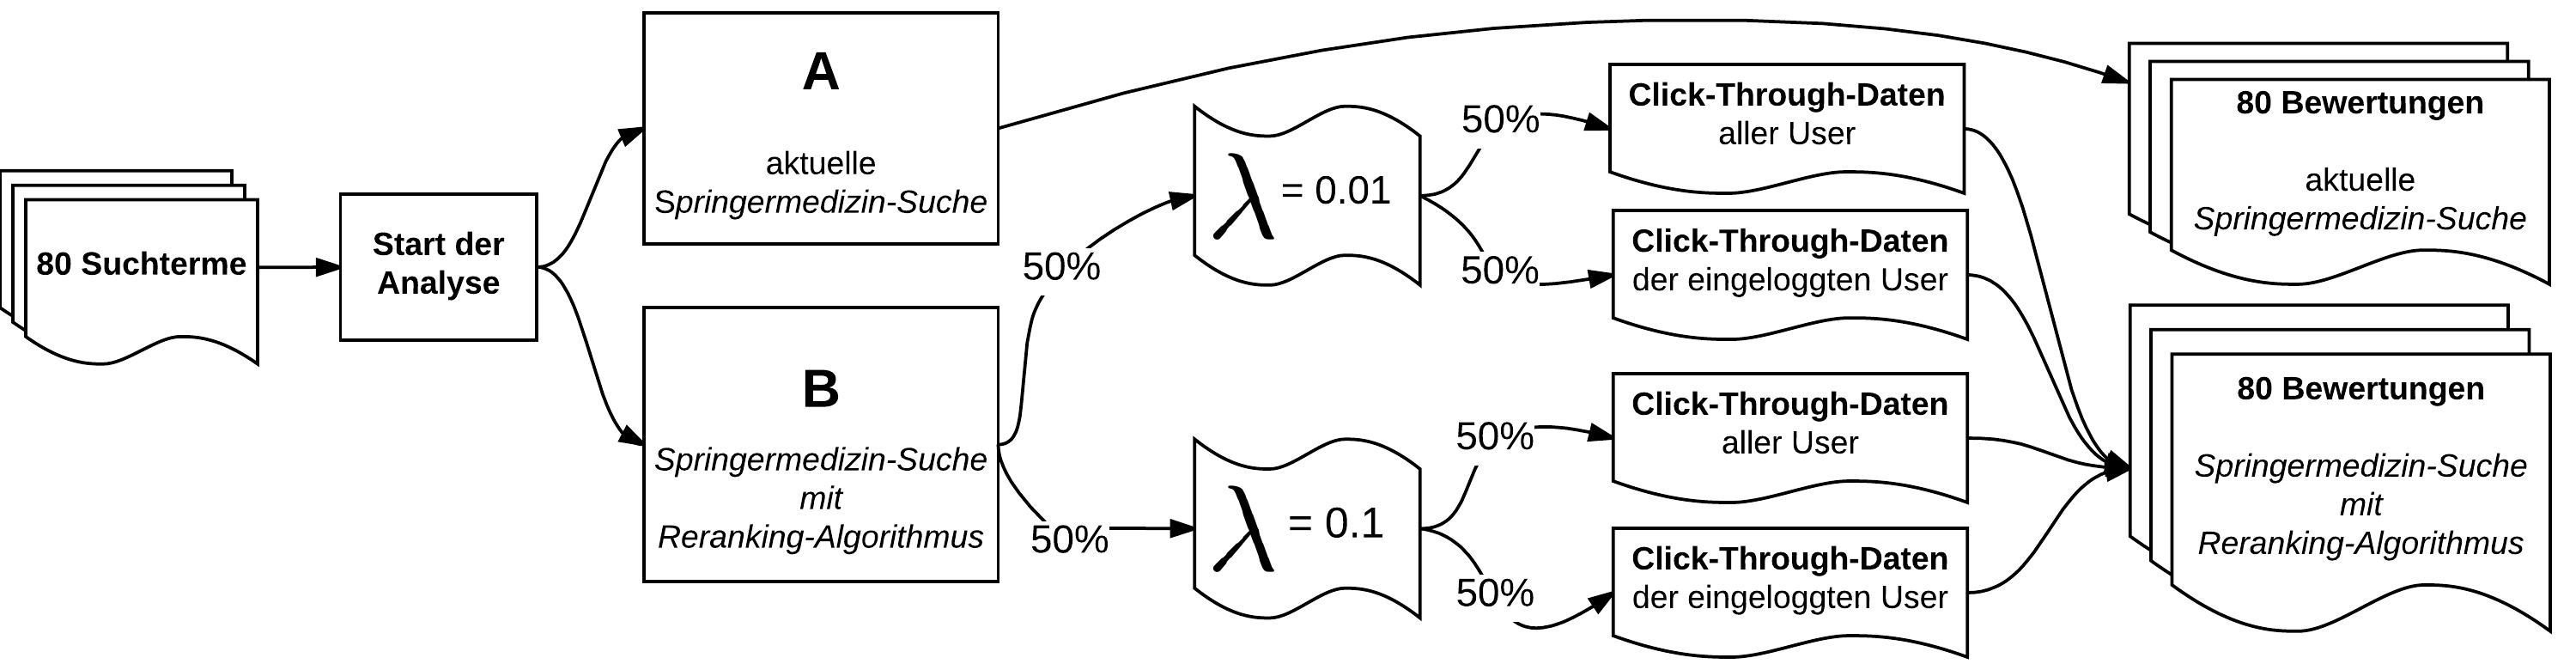
\includegraphics[width=0.7\linewidth]{gfx/EvaluationsvariantenRerankingSuche}
\vspace{-2em}
\end{figure}

\section{Auswertung der Suchergebnis-Qualität}
\label{sec:Evaluation:Auswertung}

\subsection{Quantitative Auswertung}
\label{sec:Evaluation:Auswertung:QuantitativeAuswertung}

\subsection{Diskussion}
\label{sec:Evaluation:Auswertung:Diskussion}

\section{Zusammenfassung}
\label{sec:Evaluation:Zusammenfassung}

%--------------------

%\paragraph{Manche Suchbegriffe sind aus meiner Sicht zu allgemein ( „operative Therapie“) oder veraltet („Prostata-Adenom“ statt benigne „Prostatahyperplasie“)%
